\subsection{\label{sec:results.xi1320.accept}Acceptance}

The cross sections presented in this work use an acceptance calculated from Monte Carlo (\abbr{MC}\label{abbr:mc}) simulations that include both geometry and detector response efficiency. Events were generated using a rough estimate of the excitation function of the state measured. These were fed into the tracking program (\abbr{GSIM}\label{abbr:gsim}) which converted the generated tracks into detector element hits. These hits were then smeared to mimick the observed resolution of the detector subsystems using the program \abbr{GPP}\label{abbr:gpp} which also populated the tagger using a random sampling of events from the data. The acceptance ($A$) was deterimined for each photon energy bin as the ratio of reconstructed events ($R$) to generated events ($G$):
\begin{equation}
    A = \frac{R}{G},
\end{equation}
with a standard deviation for a binomial distribution as the statistical error:
\begin{equation}
    \delta A = \sqrt{\frac{A (1 - A)}{G - 1}}.
    \label{eqn:accept.err}
\end{equation}
The number of generated events ($G$) was chosen to be large enough so that the statistical error in the accpetance is much less than the error in the flux-modified yield:
\begin{equation}
    \frac{\delta A}{A} \ll \frac{\delta Y}{Y},
\end{equation}
and $\delta A$ was added in quadrature to obtain the statistical error on the final results. The acceptance for the ground state $\Xi^-$(1320) is shown in fig.~\ref{fig:xi1320.accept}. This is applied to the flux-corrected measured yield to obtain the final excitation function, however, an investigation into the validity of this calculation is presented first in the following section.

\begin{figure}[bhp]\centering
    \includegraphics[width=0.98\columnwidth]{\figures/mmkk/xi1320_accept.eps}
    \caption[\texorpdfstring{$\Xi^-$}{Xi-}(1320) Acceptance]{\label{fig:xi1320.accept}The acceptance for the ground state $\Xi^-$(1320). Shown are the data with selections described in Tables~\ref{tab:vtime.cuts} and \ref{tab:kpkp.cuts} with and without the \abbr{TOF} energy deposit cut. The plot on the right has the added requirement of an in-time proton.}
\end{figure}

The tracking and digitizing program is not reliable along the edges of the drift chamber of \abbr{CLAS}. As a result, a fiducial cut is required to prevent a significant systematic error contribution from either gaining or loosing events that lie along these edges. This cut, shown in Fig.~\ref{fig:fidcut}, was applied to all data, real and simulated, presented in this chapter. A detailed specification of this cut is given in App.~\ref{sec:app.fidcut}.

\begin{figure}[bhtp]\centering
\begin{minipage}{0.49\linewidth}\centering
    \includegraphics[width=\columnwidth]{\figures/analysis/kp_angdisrb.eps}
\end{minipage}
\begin{minipage}{0.49\linewidth}\centering
    \includegraphics[width=\columnwidth]{\figures/analysis/kp_angdisrb_fidcut.eps}
\end{minipage}
    \caption[Fiducial Cuts]{\label{fig:fidcut}Angular distribution of the $\Kp$ tracks showing the fiducial cut. Similar cuts were made for each type of particle.}
\end{figure}



\subsection{\label{sec:results.accept.syserr}\abbr{MC} Model Dependence and Systematic Errors}

The systematic error of the acceptance, which is one of the largest sources of error for the calculated excitation functions and cross section upper limits, is the result of requiring a model to generate the simulated events. A phase-space generator is insufficient to reproduce the distributions of momenta in the data. For this analysis, a $t$-channel production via kaon exchange and a Y$^{*0}$ resonance was used to simulate the $\Xi$ production, making the parameters for event generation the mass and width of the Y$^{*0}$ and the ``$t$-slope'' of the leading K$^+$. The reaction looks like the following:

\begin{singlespacing}\begin{align}
    \gammaup \p \rightarrow & \ \Y^{*0} \Kp \nonumber \\[-0.4em]
    & \ \hookrightarrow \Xi^{-} \Kp.
    \label{rxn:xiproduction}
\end{align}\end{singlespacing}
The $t$-slope is the exponential slope constant $b$ in
\begin{equation}
    -t = a e^{-b E},
\end{equation}
where $E$ is the beam energy and $t$ is the mandelstam invariant corresponding to the momentum transfer to the leading $\Kp$:
\begin{equation}
    t = ( p^\mu_\mathrm{beam} - p^{\mu}_{\Kp} )^2
\end{equation}
An approximation of this distribution using the higher momentum $\Kp$ can been seen in the upper-left plot of Fig.~\ref{fig:simcomp.xi1320}. The values for the Y$^{*0}$ mass, width and the $t$-slope were chosen so as to mimick the distributions in the data as shown in Fig.~\ref{fig:simcomp.xi1320} and the systematic error was determined by varying them according to the features seen in the data.

\begin{figure}[bh]\centering
    \includegraphics[width=\columnwidth]{\figures/analysis/xi1320_sim_comparison.eps}
    \caption[Simulation / Data Comparion \texorpdfstring{$\Xi^-$}{Xi-}(1320)]{\label{fig:simcomp.xi1320}Comparison of simulation of the $\Xi^-$(1320) to the background-subtracted data. From left to right, top to bottom: $-t$ from the high momentum $\Kp$, cosine of the center-of-mass polar-angle ($\theta_\mathtt{CM}$) of the low momentum $\Kp$, momenta and missing mass of each $\Kp$ and the two combined ($\Kp_\mathrm{1\&2}$) and the invariant mass of $\Kp\Kp$.}
\end{figure}

The variable to which the acceptance is most sensitive is the $t$-slope of the leading $\Kp$. However, this kaon cannot be identified in the data since there are two identical $\Kp$'s in the final state. Luckily, a reasonable approximation exists using the higher momentum $\Kp$ as the leading meson in reaction~\ref{rxn:xiproduction}. The $t$-slope for this kaon as a function of beam energy is shown in Fig.~\ref{fig:measured.tslope} for both the $\Xi^-$(1320). The Y$^{*0}$ mass and width can similarly be acertained from the missing mass off the faster $\Kp$, and this is shown in Figs.~\ref{fig:mkp0.mean} and \ref{fig:mkp0.width}. The parameters used for the acceptance calculations of the $\Xi$ states are listed in Table~\ref{tab:sim.params}.

\begin{figure}[bhp]\centering
    \includegraphics[width=0.7\columnwidth]{\figures/analysis/mkp0_tslope_v_ebeam.eps}
    \caption[$\Kp_\mathrm{fast}$ $t$-slope]{\label{fig:measured.tslope}Measured $t$-slope from $\Kp_\mathrm{fast}$ for the $\Xi^-$(1320) and $\Xi^-$(1530) obtained via sideband subtraction.}
\end{figure}

\begin{figure}[tbhp]\centering
    \includegraphics[width=0.7\columnwidth]{\figures/analysis/mkp0_mean_v_ebeam.eps}
    \caption[MM($\Kp_\mathrm{fast}$) mean]{\label{fig:mkp0.mean}Mean of the missing mass off $\Kp_\mathrm{fast}$ for the $\Xi^-$(1320) and $\Xi^-$(1530) obtained via sideband subtraction.}
\end{figure}

\begin{figure}[tbhp]\centering
    \includegraphics[width=0.7\columnwidth]{\figures/analysis/mkp0_width_v_ebeam.eps}
    \caption[MM($\Kp_\mathrm{fast}$) width]{\label{fig:mkp0.width}Gaussian width ($\sigma$) of the missing mass off $\Kp_\mathrm{fast}$ for the $\Xi^-$(1320) and $\Xi^-$(1530) obtained via sideband subtraction.}
\end{figure}

\begin{table}[bhp]
\begin{minipage}{\columnwidth}
\begin{center}
\begin{singlespacing}

\caption[Simulation Parameters]{\label{tab:sim.params}The simulation parameters used to calculated the acceptance for the various $\Xi$ states.}

\begin{tabular}{lccc}

\hline \hline

 & $t$-slope & Y$^{0*}$ mass & Y$^{0*}$ width \\
 & & (GeV) & (MeV) \\

\hline

$\Xi^-$(1320) & 1.4 & 1.95 & 200 \\
$\Xi^-$(1530) & 1.7 & 2.1 & 500 \\
$\Xi^-$(1620) & 1.7 & 2.25 & 700 \\
$\Xi^-$(1690) & 1.7 & 2.5 & 1000 \\
$\Xi^-$(1820) & 1.7 & 2.7 & 1000 \\

\hline \hline

\end{tabular}

\end{singlespacing}
\end{center}
\end{minipage}
\end{table}
\vspace{20pt} % tab:sim.params

The systematic error of the acceptance coming from the Y$^{*0}$ mass, width and $t$-slope: $\delta A_{\mathrm{M}(\Y^*)}$, $\delta A_{\Gamma(\Y^*)}$ and $\delta A_{t\mbox{-}\mathrm{slope}}$ respectively, was calculated from the variance of the acceptance from events simulated using M$(\Y^*)=2.1$~GeV, $\Gamma(\Y^*) = 200$~MeV and $t$-slope$ = 2.0$ each individually and summing these in quadrature. For each of these variations, the contribution to the systematic error is given by
\begin{equation}
    \delta A^2_\mathrm{sys} = \frac{1}{N}
    \sum_i \left(
        \frac{A^\mathrm{var}_i - A_i}{A_i}
        \right)^2,
\end{equation}
where the sum is over $N$ photon energy bins, $A_i$ is the acceptance used in the excitation function calculations, and $A^\mathrm{var}_i$ is the acceptance for one of the three variations above. The comparison for each is shown in Figs.~\ref{fig:accept.syserr.a} and \ref{fig:accept.syserr.b} and results in:
\begin{align}
    \frac{\delta A_{\mathrm{M}(\Y^*)}}{A} & = 1.2 \%, \nonumber \\
    \frac{\delta A_{\Gamma(\Y^*)}}{A} & = 1.0 \%, \nonumber \\
    \frac{\delta A_{t\mbox{-}\mathrm{slope}}}{A} & = 2.3 \%.
\end{align}
Adding these in quadrature gives an estimated systematic uncertainty of 2.8\% in the acceptance. Although this study was done with the ground state $\Xi^-$(1320), it is reasonably certain to hold for each of the higher mass $\Xi$'s and is incorporated into the final results.

\begin{figure}\centering
    \includegraphics[width=0.98\columnwidth]{\figures/analysis/xi1320_accept_syserr_yresonance.eps}
    \caption[Acceptance Systematic Error, Y$^{*0}$ Properties]{\label{fig:accept.syserr.a}Acceptance for the ground state $\Xi^-$(1320) showing the effect of varying the Y$^{*0}$ mass and width.}
\end{figure}

\begin{figure}\centering
    \includegraphics[width=0.55\columnwidth]{\figures/analysis/xi1320_accept_syserr_tslope.eps}
    \caption[Acceptance Systematic Error, $t$-slope]{\label{fig:accept.syserr.b}Acceptance for the ground state $\Xi^-$(1320) showing the effect of varying the $t$-slope parameter.}
\end{figure}

There are a few more sources of systematic error that can accounted for by an overall scale factor. These include the start counter efficiency which was not included in the smearing program (\abbr{GPP}) of the simulation. This was determined to be a 6\% per track with the \emph{g11}\cite{clas.thesis.williams} experiment which had very similar running conditions including the same beam current, target and start counter. An overall efficiency that was dependent on the beam intensity was also found. This scaled linearly with the current and was approximately 16\% at 60~nA, or 0.26\% per nA. The \emph{g11} group also included a scaling factor due to multiple hits in the tagger within the same beam bucket. The last one is already accounted for in this analysis as raw tagger hits were inserted into the simulations, see Sec.~\ref{sec:analysis.beam} on page~\pageref{sec:analysis.beam}.

For the final excitation function results, a scale factor of 28\% was applied to the $\Kp\Kp$ events and 34\% was applied when a proton was detected in the event. These numbers are based on the findings of \emph{g11} and the systematic error is estimated to be 7\%. Adding this in quadrature to the 3\% error above gives a total systematic error of 8\%.




\begin{comment}
    The simulation tracking program (\abbr{GSIM}) had an inherent efficiency of approximately 90\%. The efficiency as a function of beam energy in GeV was determined to be:
    \begin{equation}
        \mathrm{\%\ Efficiency} = -1.8 E_\mathrm{beam}^2 + 5.4 E_\mathrm{beam} + 90,
        \label{eqn:gsim.eff}
    \end{equation}
    with a \emph{systematic} error of approximately $\pm5\%$, shown in Fig.~\ref{fig:gsim.eff}. This was the result of a study done by C.\ Bookwalter of the \g12 group and is still on-going at the time of this writing. Reconstructed four-momenta and the beam energy from data were input into the simulation, with all physical processes such as multiple scattering and decays turned off, and the events were analyzed once again. Comparing the original analysis to the one sent through the simulation procedure showed a loss of approximately 10\% of the tracks. The acceptances shown have been adjusted to take this effect into account.
    \begin{figure}\begin{center}
        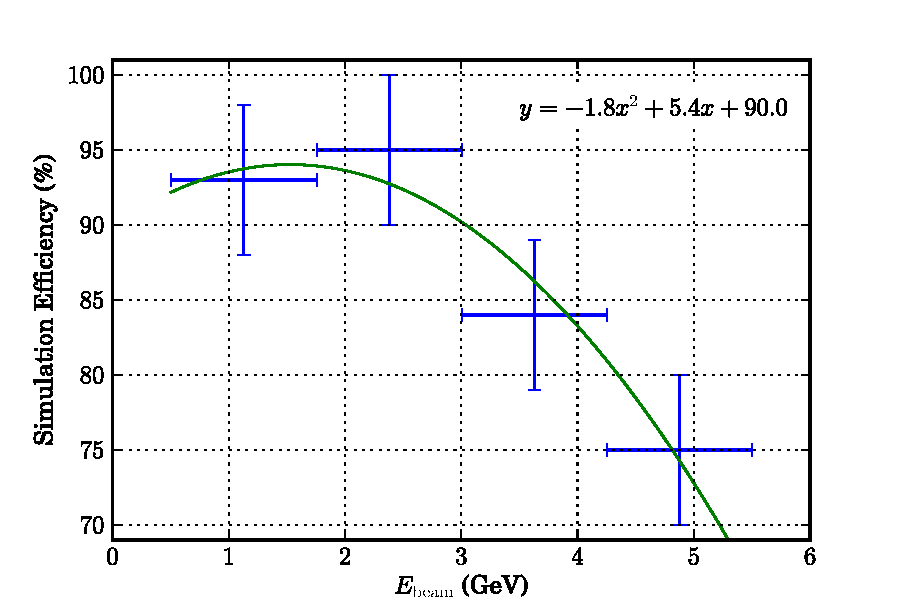
\includegraphics[width=\figwidth]{\figures/analysis/gsim_eff.eps}
        \caption[Simulation Efficiency]{\label{fig:gsim.eff}Simulation efficiency vs.\ beam energy with \emph{systematic} errors shown. The line drawn is a fitted 2\textsuperscript{nd} order polynomial with the equation shown in the upper right.}
    \end{center}\end{figure}
\end{comment}

\begin{comment}
The acceptance for the reactions

\begin{singlespacing}\begin{align}
    \gammaup \p \rightarrow & \ \Xi^-(1320) \Kp \Kp, \\
    \gammaup \p \rightarrow & \ \Xi^{*-}(1530) \Kp \Kp \nonumber \nopagebreak \\
        & \ \hookrightarrow \Xi^-(1320) \piup^0, \\
    \gammaup \p \rightarrow & \ \Xi^{*-}(1530) \Kp \Kp \nonumber \nopagebreak \\
        & \ \hookrightarrow \Xi^0(1315) \piup^-,
\end{align}\end{singlespacing}
are shown in Figs.~\ref{}
\end{comment}




\clearpage
